\documentclass[fleqn, 12pt]{article}

\usepackage[utf8]{inputenc}
\usepackage[bulgarian]{babel}
\usepackage{amsmath}
\usepackage{amssymb}
\usepackage{booktabs}
\usepackage{fancyhdr}
\usepackage{amsthm}
\usepackage{tikz}
\usepackage{centernot}

\theoremstyle{definition}
\newtheorem{example}{Пример}[subsection]
\newtheorem{definition}{Дефиниция}[subsection]
\newtheorem{axiom}{Аксиома}[subsection]
\newtheorem{theorem}{Теорема}[subsection]
\newtheorem{lemma}{Лема}[subsection]

\title{Дискретна математика \\ Упражнение}
\author{Exonaut}

\pagestyle{fancy}
\fancyhf{}
\lhead{\rightmark}
\rhead{\thepage}
\cfoot{}
\renewcommand{\headrulewidth}{0pt}

\begin{document}
\maketitle
\pagenumbering{gobble}

\newpage
\pagenumbering{arabic}

\tableofcontents
\newpage

\section{Упражнение 1: Логика и логически оператори}

\subsubsection*{Задача 1}
Кои от следните изречения са съждения? Какъв е резултатът от тези съждения?
\begin{enumerate}
\item "Китай е държава с най - много жители в света." (Съждение с резултат "Истина")
\item "София е най - големия град в света." (Съждение с резултат "Лъжа")
\item "Не пресичай улицата!" (Не е съждение, а команда)
\item "Колко е часът?" (Не е съждение, а въпрос)
\item $4 + 1 = 5$ (Съждение с резултат "Истина")
\item $4 + x = 5$ (Предикат: Истина, ако $x = 1$; Лъжа, ако $x \neq 1$)
\item $4 + x = 5$, ако $x = 1$ (Съждение с резултат "Истина")
\end{enumerate}

\subsubsection*{Задача 2}
Нека p, q, r са следните прости съждения:\\
p: "Разболяваш се." \\
q: "\textbf{Не} можеш да вземеш финалния изпит." \\
r: "Посещавал си теоретични курсове" \\
Да се опишат семантично следните комбинирани съждения:
\begin{enumerate}
\item $p \to q$ - "Ако си болен, няма да можеш да си вземеш финалния изпит."
\item $q \Leftrightarrow \neg r$ - "Няма да вземеш финалния изпит тогава и само тогава, когато не си посещавал теоретичния курс."
\item $q \to \neg r$ - "Ако не си взел финалния изпит, то тогава следва, че не си посещавал теоретичния курс."
\item $p \lor q \lor r$ - "(Ти си болен) или (не си взел финалния изпит) или (не си посещавал теоретичния курс) или и трите заедно."
\item $(p \to \neg r) \lor (q \to \neg r)$ - "(Ако си болен, тогава не си посещавал теоретичния курс) или (ако не си взел финалния изпит, тно не си посещавал теоретичния курс) - или и двете заедно."
\item $(p \land q) \lor (\neg q \land r)$ - "[(Болен си) и (не си взел финалния изпит)] или [(си взел финалния изпит) и (си посещавал теоретичния курс)]."
\end{enumerate}

\subsubsection*{Задача 3}
Нека p, q, r са следните прости съждения:\\
p: "Получил си 6 за годината." \\
q: "Решил си правилно всички домашни работи." \\
r: "Получил си 6 за всеки учебен срок." \\
Да се опишат следните комбинирани съждения с логически изрази:
\begin{enumerate}
\item  "(Получил си 6 за всеки от сроковете), но (не си решил правилно всички домашни работи)" - $r \land \neg q$
\item "(Получил си 6 за годината) и ( си решил правилно всички домашни работи) и (си получил си 6 за всеки учебен срок)." - $p \land q \land r$
\item "Ако (имаш 6 за всеки учебен срок), то (ще имаш 6 за годината)." - $ r \to q$
\item "(Получил си 6 за всеки учебен срок), но (не си решил правилно всички домашни работи), но въпреки това (си получил 6 за годината)." - $r \land  \neg q \land p$
\item "(Получаването на 6 за всеки учебен срок) и (правилното решаване на всички домашни работи) е достатъчно условие за (получаване на 6 за годината)." - $(r \land q) \to p$
\item "(Ти си получил 6 за годината) тогава и само тогава когато [(си решил  правилно всички домашни работи) и (си получил 6 за всеки учебен срок)]." - $р \Leftrightarrow (q \land r)$ 
\end{enumerate}

\subsubsection*{Задача 4}
Да се състави таблица на истинност за следните комбинирани съждения:
\begin{enumerate}
\item $\neg p \otimes \neg p$
\item $(p \lor q) \land \neg r$
\item $(p \to q) \to r$
\item $(p \land \neg q) \Leftrightarrow (p \land r)$
\end{enumerate}
Решение: 
\begin{enumerate}
\item $\neg p \otimes \neg p$
\begin{table}[htp]
  \begin{center}
    \begin{tabular}{|c|c|c|c|c|} 
\hline
      \textbf{p} & \textbf{q}  & \textbf{ $\neg p$ } & \textbf{$\neg q$} & \textbf{ $\neg p \otimes \neg p$}\\
      \hline
	F & F & T & T & F\\
\hline
	F & T & T & F & T\\
\hline
	T & F & F  & T & T\\
\hline
 	T & T & F  & F & F\\
\hline
    \end{tabular}
  \end{center}
\end{table}

\item $(p \lor q) \land \neg r$
\begin{table}[htp]
  \begin{center}
    \begin{tabular}{|c|c|c|c|c|c|} 
\hline
      p & q  &  r & $p \lor q$ & $\neg r$ & $(p \lor q) \land \neg r$\\
      \hline
	F & F & F & F & T & F\\
\hline
	F & F & T & F & F & F\\
\hline
	F & T & F  & T & T & T\\
\hline
 	F & T & T  & T & F & F\\
\hline
	T & F & F & T & T & T\\
\hline
	T & F & T & T & F & F\\
\hline
	T & T & F  & T & T & T\\
\hline
 	T & T & T  & T & F & F\\
\hline
    \end{tabular}
  \end{center}
\end{table}
\newpage
\item $(p \to q) \to r$
\begin{table}[htp]
  \begin{center}
    \begin{tabular}{|c|c|c|c|c|} 
\hline
      p & q  & $p \to q$  & r & $(p \to q) \to r$\\
      \hline
	F & F & T & F & F\\
\hline
	F & F & T & T & T\\
\hline
	F & T & T  & F & F\\
\hline
 	F & T & T  & T & T\\
\hline
	T & F & F & F & T\\
\hline
	T & F & F & T & T\\
\hline
	T & T & T  & F & F\\
\hline
 	T & T & T  & T & T\\
\hline
    \end{tabular}
  \end{center}
\end{table}

\item $(p \land \neg q) \Leftrightarrow (p \land r)$
\begin{table}[htp]
  \begin{center}
    \begin{tabular}{|c|c|c|c|c|c|c|} 
\hline
      p & q  &  r & $ \neg q$ & $p \land \neg q$ & $p \land r$ & $(p \land \neg q) \Leftrightarrow (p \land r)$\\
      \hline
	F & F & F & T & F & F & T\\
\hline
	F & F & T & T & F & F & T\\
\hline
	F & T & F  & F & F & F & T\\
\hline
 	F & T & T  & F & F & F & T\\
\hline
	T & F & F & T & T & F & F\\
\hline
	T & F & T & T & T & T & T\\
\hline
	T & T & F  & F & F & F & T\\
\hline
 	T & T & T  & F & F & T & T\\
\hline
    \end{tabular}
  \end{center}
\end{table}
\end{enumerate}

\subsubsection*{Задача 5}
Да се докаже по 2 начина, че всеки от следните логически изрази е тавтология:\\
1. Чрез таблица на истинност. \\
2. Чрез закони за еквивалентно преобразувание. \\
\begin{enumerate}
\item $(p \land q) \to q$
\item $[\neg p \land (p \lor q)] \to q$
\item $[p \land (p \to q)] \to q$
\end{enumerate}
Решение:
\begin{enumerate}
\item $(p \land q) \to q$
\begin{table}[htp]
  \begin{center}
    \begin{tabular}{|c|c|c|c|} 
\hline
      p & q  & $p \land q$  & $(p \land q) \to q$  \\
      \hline
	F & F & F & T \\
\hline
	F & T & F & T\\
\hline
	T & F & F  & T \\
\hline
 	T & T & T  & T \\
\hline
    \end{tabular}
  \end{center}
\end{table}
\begin{gather*}
(p \land q) \to q \\
\Leftrightarrow \neg(p \land q) \lor q \quad \text{(закон за импликация)} \\
\Leftrightarrow (\neg p \lor q) \land q \quad\text{(закон на де Морган)} \\
\Leftrightarrow \neg p \lor (\neg q \lor q) \quad \text{(асоциативен закон)} \\
\Leftrightarrow \neg p \lor T \quad \text{(закон за тривиална тавтология)} \\
\Leftrightarrow T \quad \text{(закон за доминиране)} \\
\end{gather*}
\item $[\neg p \land (p \lor q)] \to q$
\begin{table}[htp]
  \begin{center}
    \begin{tabular}{|c|c|c|c|c|c|} 
\hline
      p & q  & $ \neg p$  & $p \lor q$ & $\neg p \land (p \lor q)$ & $[\neg p \land (p \lor q)] \to q$\\
      \hline
	F & F & T & F &F & T\\
\hline
	F & T & T & T & T &T \\
\hline
	T & F & F  & T & F & T \\
\hline
 	T & T & F  & T & F & T \\
\hline
    \end{tabular}
  \end{center}
\end{table}
\begin{gather*}
[\neg p \land (p \lor q)] \to q \\
\Leftrightarrow \neg [\neg p \land (p \lor q)] \lor q  \quad \text{(закон за импликация)} \\
\Leftrightarrow [\neg \neg p \lor (p \lor q)] \lor q \quad\text{(закон на де Морган)} \\
\Leftrightarrow [ p \lor \neg(p \lor q)] \lor q \quad \text{(закон за двойното отрицание)} \\
\Leftrightarrow  (p \lor q) \lor \neg (p \lor q) \quad \text{(асоциативен закон)} \\
\Leftrightarrow T \quad \text{(закон тривиална тавтология)} \\
\end{gather*}
\item $[p \land (p \to q)] \to q$
\begin{table}[htp]
  \begin{center}
    \begin{tabular}{|c|c|c|c|c|} 
\hline
      p & q  & $ p \to q$  & $p \land (p \to q) $ & $[p \land (p \to q)] \to q$ \\
      \hline
	F & F & T & F &T \\
\hline
	F & T & T & F & T  \\
\hline
	T & F & F  & F & T  \\
\hline
 	T & T & T  & T & T \\
\hline
    \end{tabular}
  \end{center}
\end{table}
\begin{gather*}
[p \land (p \to q)] \to q\\
\Leftrightarrow [p \land (\neg p \lor q)] \to q  \quad \text{(закон за импликация)} \\
\Leftrightarrow [(p \land \neg p) \lor (p \land q)] \to q \quad\text{(дистрибутивен закон)} \\
\Leftrightarrow [F \lor (p \land q)] \to q\quad \text{(закон за тривиално опровержение)} \\
\Leftrightarrow (p \land q) \to q  \quad \text{(комутативен закон и закон за идентичност)} \\
\Leftrightarrow T \quad \text{(доказано в 1.)} \\
\end{gather*}
\end{enumerate}

\newpage
\section{Упражнение 2: Предикати и предикатни функции}

\subsubsection*{Задача 1}
Нека $P(x,y)$ е  предикатна  функция,  съответстваща  на  следното твърдение $x + 2y = x+y$, където x и y са цели числа.  Какъв е резултатът от:
\begin{enumerate}
\item $P(1,-1)$
$$P(1,-1) \Leftrightarrow 1 + 2 \cdot (-1) = 1 - 1  \Leftrightarrow -1 = 0 \quad \text{Лъжа}$$  
\item $P(0,0)$
$$P(0,0) \Leftrightarrow 0 + 2 \cdot 0= 0 + 0  \Leftrightarrow 0 = 0 \quad \text{Истина}$$  
\item $P(2,1)$
$$P(2,1) \Leftrightarrow 2 + 2 \cdot 1 = 2 + 1 \Leftrightarrow 4 = 3 \quad \text{Лъжа}$$  
\end{enumerate}

\subsubsection*{Задача 2}
Нека $Q(x)$ е предикатна функция, съответстваща на следното твърдение $x+1 = 2x$, където x е реално число.  Какъв е резултатът от:
\begin{enumerate}
\item $Q(2)$
$$Q(2) \Leftrightarrow 2+1 = 2 \cdot 2 \Leftrightarrow 3 = 4 \quad \text{Лъжа}$$  
\item $\forall x Q(x)$
$$\forall x Q(x) \implies \quad \text{Лъжа}$$  
\item $\exists x Q(x)$
$$\exists x Q(x) \Leftrightarrow \exists x = 1 \text{ което е решение на } Q(x)$$  
\end{enumerate}

\subsubsection*{Задача 3}
Нека $R(x)$ е предикатна функция, съответстваща на следното твърдение: "ако $x+3 = 6$, то $x + 8 = 16$". Какъв е резултатът от:
\begin{enumerate}
\item $R(3)$
$$3 + 3 = 6 \, T \quad 3+8 = 16 \, F \implies \text{ Лъжа}$$  
\item $R(8)$
$$8 + 3 = 6 \, F \quad 8+8 = 16 \, T \implies \text{ Истина}$$  
\item $R(2)$
$$2 + 3 = 6 \, F \quad 2+8 = 16 \, F \implies \text{ Истина}$$  
\item $\exists (x)(R(x)) \quad x \in \mathbb{Z}$
$$x + 3 = 6, x=3 \, T \quad 3+8 = 16 \, F \implies \text{ Лъжа}$$  
\end{enumerate}

\subsubsection*{Задача 4}
Нека е известно: \\
X -  множеството на всички хора, \\
$x \in X$\\
C(x) е предикат: "x е комик" \\
F(x) е предикат:  "x умее да разказва смешни истории" \\
Да се опишат семантично следните комбинирани предикати:
\begin{enumerate}
\item $\exists x C(x)$ - "Съществува човек, който е комик."
\item $\exists x \neg C(x)$ - "Не всеки човек е комик." или " Съществува човек, който не е комик."
\item $\forall x \neg C(x)$ - "Всеки човек е комик."
\item $\neg \forall x C(x)$ - "Никой не е комик."
\item $\exists x \neg F(x)$ - "Съществува човек, който не умее да разказва смешни истории."
\item $\forall x \neg F(x)$ - "Никой (нито един човек) не умее да разказва смешни истории."
\item $\forall x (C(x) \to F(x))$ - "Всеки  човек, който  е  комик, умее  да  разказва  смешни истории."
\item $\exists x (C(x) \land \neg F(x))$ - "Съществува човек, който е комик, но не умее да разказва смешни истории."
\item $\exists x (F(x) \land \neg C(x))$ - "Съществува човек, който умее да разказва смешни истории, но не е комик."
\item $\forall x (C(x) \land F(x))$ - "Всеки човек е комик и умее да разказва смешни истории."
\item $\exists x (C(x) \land F(x))$ - "Съществува човек, който е комик и умее да разказва смешни истории."
\end{enumerate}

\subsubsection*{Задача 5}
Ако с X е означено множеството навсички студенти от ФКСУ, нека са известни следните предикати:\\
$P(x)$: "x е взел изпита по ДС" , \\
$Q(x)$: "x знае да програмира на езика C ++".   \\
Опишете  чрез  логически  изрази  следните  комбинирани  предикати,  на  простите предикати  P(x) и   Q(x), изпо лзвайки кванторите за общност и съществуване  $\forall \text{ и } \exists$ и необходимите логически оператори. 
\begin{enumerate}
\item "Съществува студентот ФКСУ, който е взел изпита по ДС и знае  да програмира на езика C ++." - 
$\exists x(P(x) \land Q(x))$
\item "Съществува студентот ФКСУ,който не знае да програмира на езика C++, но е взел изпита по ДС." - 
$\exists x(P(x) \land \neg Q(x))$
\item "Всички студенти от ФКСУ, които знаят да програмират на езика С++, са взели изпита по ДС."  - 
$\forall x(Q(x) \to P(x))$
\item "Само някои от студентитеот ФК СУ, които знаят да програмират на езика С++, са взели из   пита по ДС." - 
$\exists x(Q(x) \to P(x))$
\item "Всички студенти от ФКСУ знаят да програмират на езика С++ ИЛИса взели изпита по ДС."-
$\forall x(P(x) \lor Q(x))$
\end{enumerate}

\subsubsection*{Задача 6}
Да се определи резултатът от следните твърдения: 
\begin{enumerate}
\item $\exists x(x^3 = -1 \land x \in \mathbb{R})$
$$\exists x(x^3 = -1 \land x \in \mathbb{R}) \Leftrightarrow x = -1 \in \mathbb{R} \implies \text{ Истина}$$  
\item $\exists x(x^3 = -1 \land x \in \mathbb{N})$
$$\exists x(x^3 = -1 \land x \in \mathbb{N}) \Leftrightarrow x = -1 \notin \mathbb{N} \implies \text{ Лъжа}$$  
\item $\forall x(2x > x \land x \in \mathbb{R})$
$$\forall x(2x > x \land x \in \mathbb{R}) \Leftrightarrow x>0 \land x \in R \implies \text{ Лъжа} $$  
\item $\forall x(2x \geq x \land x \in \mathbb{N})$
$$\forall x(2x > x \land x \in \mathbb{R}) \Leftrightarrow x \geq 0 \land x \in R \implies \text{ Истина} $$  
\end{enumerate}
\newpage
\section{Упражнение 3: Теория на множествата}

\subsubsection*{Задача 1}
Нека А е универсалното множество, а\\
$F(A)$ е предикат "A е крайно множество.",  \\
$I(A)$ е предикат " A е безкрайно множество.", \\
$S(A, B)$ е предикат " A се съдържа в B.", \\
$E(A)$ е предикат "Aе празно множество."  \\
Да се запишат с логически изрази следните съждения:\\
\begin{enumerate}
\item "Не всички множества са крайни."
$$\exists A I(A) \qquad \exists A \neg F(A)$$
\item "Всяко подмножество на крайно множество е крайномножество." 
$$\exists A \exists B [(S(A,B) \land F(B)) \to F(A)]$$
\item "Никое безкрайно множество не се съдържа в крайно множество."
$$\exists A \exists B [(I(A) \land S(A,B) \land F(B)) \to \varnothing]$$
\item "Празното множество е подмножество на всяко крайно множество." 
$$\exists A \exists B [(E(A) \land F(B)) \to S(A,B)]$$
\item "Празното множество е подмножество на всяко безкрайно множество."
$$\exists A \exists B [(E(A) \land I(B)) \to S(A,B)]$$
\end{enumerate}

\subsubsection*{Задача 2}
Да се запишат членовете на всяко от следните множества:
\begin{enumerate}
\item $X\{x \vert x \in \mathbb{Z} \land x^2 = 4 \} = \{-2,2\}$
\item $X\{x \vert x \in \mathbb{N} \land x^2 = 4 \} = \{2\}$
\item $X\{x \vert x \in \mathbb{Z} \land x^2 = 5 \} = \{\} = \varnothing$
\item $X\{5x \vert x \in \mathbb{Z} \land -2 \leq x^2 \leq 2\} = \{-5,0,5\}$
\item $X\{x \vert x \in \mathbb{N} \land x^2 \in \{1, 4, 9\} \} = \{ 1,2,3\}$
\item $X\{x \vert x \in \mathbb{Z} \land x^2 \in \{1, 4, 9\} \} = \{ -3,-2,-1,1,2,3\}$
\end{enumerate}

\subsubsection*{Задача 3}
Да  се  запишат  посочените  множества  чрез  използване  на  функция  на принадлежност към даденото множество
\begin{enumerate}
\item $X = \{0,3,6,9,12 \} = \{3x \vert x \in Z  \land 0 \leq x \leq 4 \}$
\item $X = \{-3,-2,-1,0,1,2,3 \} = \{x \vert x \in Z  \land \vert x \vert \geq 3 \}$
\item $X =\{1,4,8,16,25,36,49 \} = \{x^2 \vert x \in Z \land  -7 \leq x \leq 7 \land x \neq 0\}$
\end{enumerate}
\subsubsection*{Задача 6}
Истина ли е твърдението $A - (B \cap C) = (A-B) \cup (A - C)$
$$A - (B \cap C) = A \cap \neg(B \cap C) = A \cap ( \neg B \cap  \neg C) = (A \cap \neg B) \cup (A \cap  \neg C) = (A-B) \cup (A - C)$$
\subsubsection*{Задача 7}
Истина ли е твърдението $A - (B \cap C) = (A-B) \cap (A - C)$
$$A - (B \cap C) = (A-B) \cup (A - C) [\text{ зад. 6}] \neq (A-B) \cap (A - C) $$
\newpage
\subsubsection*{Задача 4}
\begin{figure}[h!]
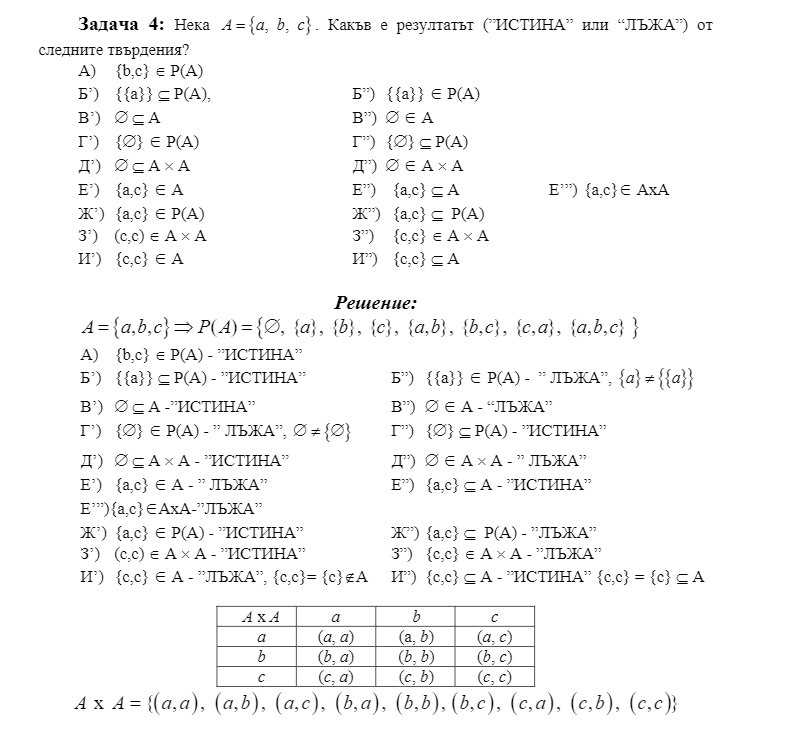
\includegraphics{Pics/Discrete math/ex3/ex3-task4.png}
\end{figure}

\newpage
\begin{figure}[htp!]
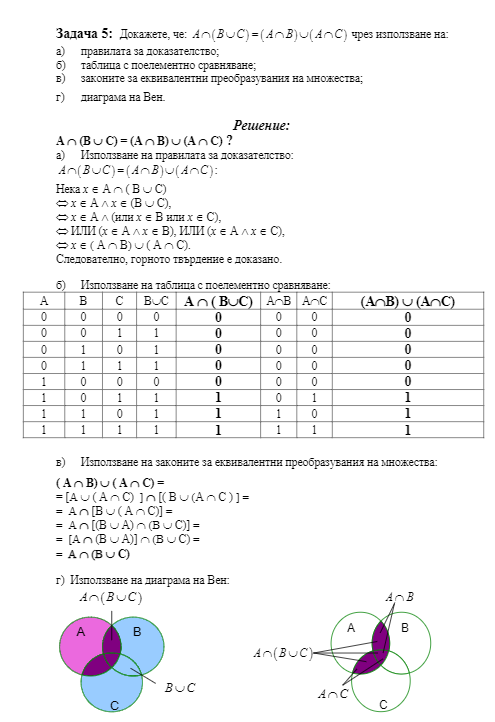
\includegraphics{Pics/Discrete math/ex3/ex3-task5.png}
\end{figure}

\newpage
\subsubsection*{Задача 9}
Истина или лъжа е следното твърдение $A \otimes (B \otimes C) = (A \otimes B) \otimes C$
\begin{table}[htp]
\begin{center}
\begin{tabular}{|c|c|c|c|c|c|c|} 
\hline
 A & B & C  & $A \otimes B$ & $B \otimes C$ & $A \otimes (B \otimes C)$ & $(A \otimes B) \otimes C$  \\
\hline
0 & 0 & 0 & 0 & 0 & 0 & 0 \\
\hline
0 & 0 & 1 & 0 & 1 & 1 & 1 \\
\hline
0 & 1 & 0 & 1 & 1 & 1 & 1 \\
\hline
0 & 1 & 1 & 1 & 0 & 0 & 0 \\
\hline
1 & 0 & 0 & 1 & 0 & 1 & 1 \\
\hline
1 & 0 & 1 & 1 & 1 & 0 & 0 \\
\hline
1 & 1 & 0 & 0 & 1 & 0 & 0 \\
\hline
1 & 1 & 1 & 0 & 0 & 1 & 1 \\
\hline
\end{tabular}
\end{center}
\end{table}
\newpage

\subsubsection*{Задача 10}
Какъв ще е резултатът от следните твърдения?
\begin{enumerate}
\item $A - (B - C) = (A - B) - C$
\item $(A-C) - (B-C) = A - B$
\item $A \cup (B \cap C) = (A \cup B) \cap (A \cup C)$
\item $A \cap (B \cup C) = (A \cap B) \cup (A \cap C)$
\item $A\cup C = B \cup C \implies A = B$
\item $A\cap C = B \cap C \implies A = B$
\item $A \otimes B = A \implies B =A$
\end{enumerate}

\begin{figure}[h!]
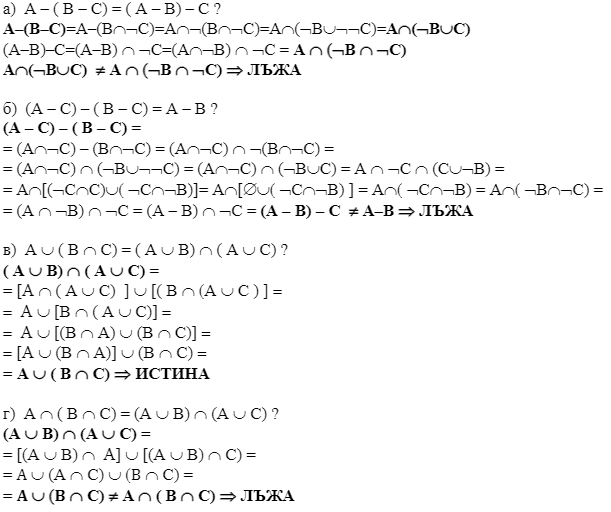
\includegraphics{Pics/Discrete math/ex3/ex3-task10-1.png}
\end{figure}

\begin{figure} 
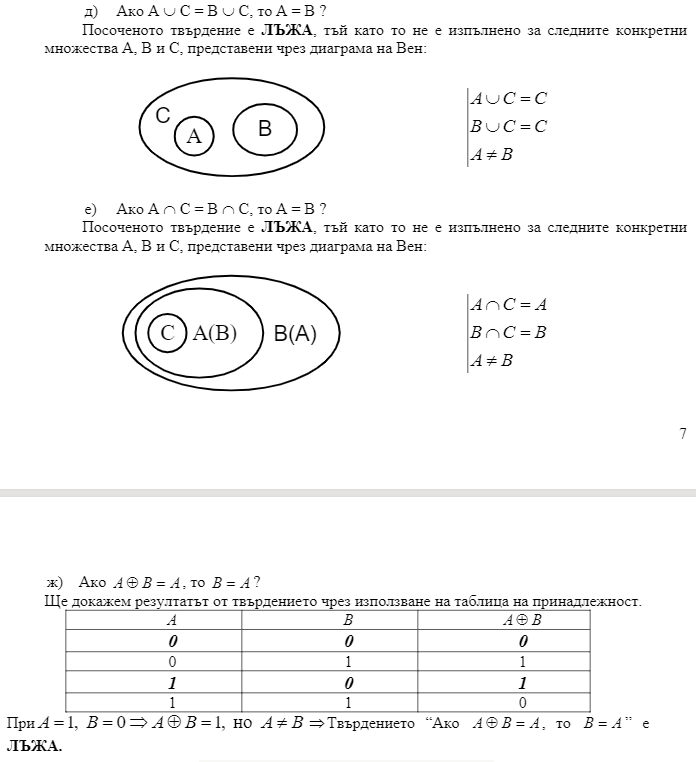
\includegraphics{Pics/Discrete math/ex3/ex3-task10-2.png}
\end{figure}

\newpage
\section{Упражнение 4: Математически доказателства}

\subsubsection*{Задача 1}
За  всеки  от  следващите  аргументи  кои  правила  за  доказателство  са използвани на всяка стъпка?
\begin{enumerate}
\item "Студентката от ТУ-София Петя има собствена кола. Всеки, който има кола, пътува по-удобно и по-бързо. Следователно, съществува студент от ТУ-София, който пътува по-удобно и по-бързо."
\item "Всеки от петимата студенти от ТУ-София Иван, Георги, Петър, Стоян и Никола е взел успешно изпита по ТЕ-1.  Всеки студент, който е взел успешно ТЕ-1 има право да се яви на изпит по ТЕ-2. Следователно, и петте гореспоменати момчета могат да се явят на изпит по ТЕ-2 през лятната сесия."
\end{enumerate}
Решение:
\begin{enumerate}
\item Нека: X - множество на всички студенти, x- произволен студент\\
c(x) - "х е студент от ТУ-София."\\
p(x) - "х    има собствена кола"\\
s(x) - "x се придвижва по-удобно и по-бързо."\\
Доказателство: \\
Изходни хипотези: c(Петя), p(Петя) и$\forall x( p(x) \to s(x) )$. \\
Заключение:$\exists x( c(x) \land s (x) )$.
\begin{enumerate}
\item $\forall x( p(x) \to s(x) ) \quad$ Хипотеза
\item p(Петя) $\to$ s(Петя) $\quad$ Универсално следствие (Universal instantiation) от а
\item p(Петя) $\quad$ Хипотеза
\item s(Петя) $\quad$ Закон на безразличие (Modus Ponens) от б и в 
\item c(Петя) $\quad$ Хипотеза
\item c(Петя) $\land$ s(Петя)  $\quad $ Конюнкция ( Conjunction)от г и д 
\item $\exists x( c(x) \land s (x) ) \quad$ Частично обобщение (Existential generalisation) от е
\end{enumerate}
\item Нека: X  – множест  во от всички студенти в ТУ-София; x  – произволен студентот X.\\ 
f(x) - "x е един от петимата студенти Иван, Георги, Петър, Стоян и Никола."\\
$t_1(x)$ - "x е взел успешно изпита по ТЕ-1."\\
$t_2(x)$ - "x има право да се яви на изпит по ТЕ-2."\\
y - произволен студент от петиматапо-горе. \\
Изходни хипотези:$\forall x(f(x) \to t_1(x))$ и$\forall x(t_1(x) \to  t_2(x))$ \\
Заключение:$\forall x(f(x) \to t_2(x))$. \\
Доказателство:
\begin{enumerate}
\item $\forall x(f(x) \to t_1(x)) \quad $ Хипотеза 
\item $f(y) \to t_1(x) \quad $ Универсално следствие (Universal instantiation) от а
\item $\forall x(t_1(x) \to  t_2(x)) \quad  $ Хипотеза
\item $t_1(y) \to  t_2(y) \quad $ Универсално следствие (Universal instantiation) от в
\item $f(y) \to  t_2(y) \quad $ Хипотетичен силогизъм (Hypothetical syllogism) от б и г
\item $\forall x(f(x) \to t_2(x)) \quad $ Универсално обобщение (Universal generalisation) от д 
\end{enumerate}
\end{enumerate}

\subsubsection*{Задача 2}
Коректно ли е доказателството на следния аргумент: "Ако $n^2$ не се дели на 3, то n също не е кратно на 3?"\\ Доказателство: " Ако $n^2$ не се дели на 3, тогава $n^2 \neq 3k, k =0, 1, ...$. Следователно $n \neq 3l, l=0, 1, ...$, откъдето следва, че n не е кратно на 3."\\
Решение \\
От  горното  доказателство  се  вижда,  че  от  това,  че $n^2 \neq 3k, k =0, 1, ...$ не  следва директно, че $n \neq 3l, l=0, 1, ...$ а трябва да се докаже. \\
За целта ще използваме индиректно доказателство: “Ако n е кратно на 3, то $n^2$ също се дели на 3.” \\
Ако допуснем, че n е кратно на 3 $\implies$ 
$$n = 3l \implies n^2 = (3l)^2 = 3(3l)^2 = 3k \implies n^2$$
Откъдето следва, че горепосоченият аргумент е верен, но посоченото доказателство е некоректно.

\subsubsection*{Задача 3}
Да се докаже, че квадратът на всяко четно число е също четно число чрез:
\begin{enumerate}
\item директно доказателство
\item индиректно доказателство
\item използване на контра-пример
\end{enumerate}
Хипотеза p : "n е четно число."
Заключение q: "$n^2$ е четно число."
\begin{enumerate}
\item директно доказателство $p \to q$\\
Нека n е  четно  число $\implies$ то  може  да  се  запише  като:
$$n = 2k, k =0, 1, ... \implies n^2 = (2k)^2 = 4k^2 = 2(2k^2) \implies n^2$$ 

\item индиректно доказателство $(\neg p \to \neg q) \Leftrightarrow (p \to q)$\\
Нека $n^2$ е нечетно число $\implies$ то може да се запише като: 
$$n^2 = 2k+1, k =0, 1, ... $$
$\implies$  n е нечетно число.

\item използване на контра-пример \\
"Ако $n^2$ е нечетно число, то nсъщо е нечетно число." \\
Хипотеза 1: "$n^2$ е нечетно число." - p \\
Хипотеза 2:  "n е четно число." -  $\overline{q} $\\
Допускаме, че Хипотеза 2 $\overline{q} $ е вярна $\implies$
$$n =2k, k =0, 1, ... \implies n^2 = (2k)^2 = 2(2k^2) \implies n^2 = 2l \implies n^2$$
 e четно число, т.е. $\overline{p} $, което е в противоречие с Хипотеза 1 p $\implies$
Допускането е грешно $\implies$ Хипотеза 2 не е вярна $\implies$ "n е нечетно число."
\end{enumerate}

\subsubsection*{Задача 4}
Да се докаже, че произведението на две рационални числa е също рационално числo.\\
Решение \\
Директно доказателство: Нека а и b са рационални числа $\implies$ те могат да се запишат във вида 
$$a = \frac{k}{l} \quad b = \frac{s}{t} \qquad k,l,s,t \in \mathbb{Z}, l \neq 0, s \neq 0 \implies ab = \frac{ks}{lt}$$

\subsubsection*{Задача 5}
Вярно е, че произведението на две ирационални числа е ирационално число?\\
Решение\\
Aко $a = b = \sqrt{2} \implies ab = 2$ което е рационално число $\implies$ твърдението е лъжа.

\subsubsection*{Задача 6}
Да се докаже, че следващите три твърдения са еквивалентни при $n \in Z$.
\begin{enumerate}
\item n е четно число.
\item n+1 е нечетно число.
\item 3n+1 е нечетно число.
\end{enumerate}
$1 \to 2$\\
$$n = 2k \implies n+1 = 2k + 1 , k \in \mathbb{N}$$
$2 \to 3$\\
$$n+1 = 2k + 1 \implies 3n + 1 = 3(2k) + 1 = 2(3k) + 1 = 3n + 1, k \in \mathbb{N}$$
$3 \to 1$\\
$$3n + 1 = 2k + 1 \implies 3n = 2k, 2k = 2t \implies n = 2k , k,t \in \mathbb{N}$$

\subsubsection*{Задача 7}
Да се докаже, че $\sqrt[3]{3}$ е ирационално число! \\
Решение\\
$a \in \mathbb{Z}, b \in \mathbb{Z}$ a,b - взаимно прости(Най голям общ делител = 1)\\
$$\frac{a}{b} = \sqrt[3]{3} \implies \left( \frac{a}{b}\right)^3 = 3 \implies a^3 = 3b^3$$
$a^3$ е кратно на 3 $\implies$ a се дели на 3 $\implies$
$$a = 3k, k \in \mathbb{N} \implies 3b^3 = a^3 = (3k)^3 = 9k^3 \implies b^3 = 9k^3 = 3s, s \in \mathbb{N}$$
$b^3$ е кратно на 3 $\implies$ b се дели на 3 $\implies$
$$b = 3l, l \in \mathbb{N} \implies \frac{a}{b} = \frac{3k}{3l} \implies$$
a и b не са взаимно прости числа (най-големият им общ делител е 3), както допуснахме по-горе $\implies$ Хипотезата, e лъжа $\implies$ $\sqrt[3]{3}$ е ирационално число

\newpage
\section{Упражнение 5: Булева алгебра}

\subsubsection*{Задача 1}
Нека функцията $f(x,y,z)$ е дефинирана посредством следната таблица:
\begin{table}[htp]
\begin{center}
\begin{tabular}{|c|c|c|c|c|} 
\hline
  &  &   & а  & б \\
\hline
x & y & z & f(x,y,z) & f(x,y,z) \\
\hline
0 & 0 & 0 & 1 & 0 \\
\hline
0 & 0 & 1 & 0 & 1 \\
\hline
0 & 1 & 0 & 1 & 0 \\
\hline
0 & 1 & 1 & 0 & 0 \\
\hline
1 & 0 & 0 & 0 & 1 \\
\hline
1 & 0 & 1 & 0 & 1 \\
\hline
1 & 1 & 0 & 1 & 0 \\
\hline
1 & 1 & 1 & 1 & 1 \\
\hline
\end{tabular}
\end{center}
\end{table}
Да се намери съответни аналитични изрази!  \\
a) $f(x,y,z) = (-x) \cdot (-y) \cdot (-z) +(-x) \cdot y \cdot (-z) + x \cdot y \cdot (-z) + x \cdot y \cdot z$  \\
б) $f(x,y,z) = (-x) \cdot (-y) \cdot z + x \cdot (-y) \cdot(-z) + x \cdot (-y) \cdot z + x \cdot y \cdot z$
\subsubsection*{Задача 2}
Истина или лъжа са следните твърдения 
\begin{enumerate}
\item $(a \vert b = b \vert a) \Leftrightarrow a = b$ 
\begin{table}[htp]
\begin{center}
\begin{tabular}{|c|c|c|c|} 
\hline
a & b & $a \vert b$ & $b \vert a$\\
\hline
0 & 0 & 1 & 1 \\
\hline
0 & 1 & 1 & 1 \\
\hline
1 & 0 & 1 & 1 \\
\hline
1 & 1 & 0 & 0 \\
\hline
\end{tabular}
\end{center}
\end{table}
\item $(a \vert b) \cdot (c \vert d) \Leftrightarrow (a+c) \vert (b+d) $
\begin{equation}
(a \vert b) \cdot (c \vert d) =
 (\overline{a \cdot b}) \cdot (\overline{c \cdot d}) = 
(\overline{a} + \overline{b}) \cdot (\overline{c} + \overline{d}) = 
\overline{a} \cdot \overline{c} + \overline{a} \cdot \overline{d} + \overline{b} \cdot \overline{c} + \overline{b} \cdot \overline{d}
\end{equation}
\begin{equation}
(a+c) \vert (b+d) = 
\overline{(a+c) \cdot (b+d)} =
\overline{a+c} + \overline{b + d} = 
\overline{a} \cdot \overline{c} + \overline{b} \cdot \overline{d}
\end{equation}
От (1) и (2) $\implies (a \vert b) \cdot (c \vert d) \neq (a+c) \vert (b+d)$
\end{enumerate}
\newpage
\section{Упражнение 6: Релации }

\subsubsection*{Задача 1}
Да се провери дали всяка от бинарните релации е\\
рефлексивна/антирефлексивна/симетрична/асиметрична/антисиметрична/транзитивна:
\begin{enumerate}
\item Релация R върху множествотo N, където $(a,b) \in R $ тогава и само тогава когато $a \land b$
\begin{figure} [htp!]
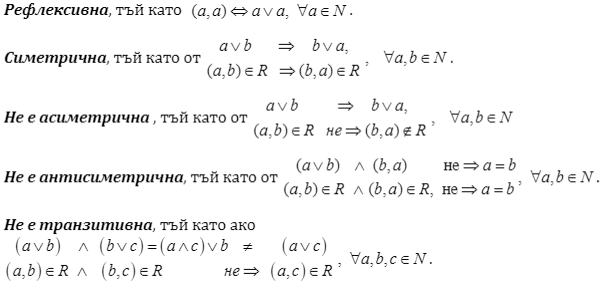
\includegraphics[width=\linewidth]{Pics/Discrete math/ex6/ex6-task1-1.png}
\end{figure}
\item Релация R върху множеството S = \{w,x,y,z \}, където 
$$R = \{ (w, w), (w, x), (x, w), (x, x), (x, z), (y, y), (z, y), (z, z) \}$$
\begin{figure} [htp!]
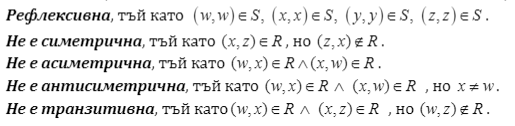
\includegraphics[width=\linewidth]{Pics/Discrete math/ex6/ex6-task1-2.png}
\end{figure}
\item Релация R върху множеството $P(x)$ на  множеството X = \{ 1, 2, 3, 4\} където $(S,T) \in R$ тогава и само тогава когато $S \subseteq T$
\begin{figure} [htp!]
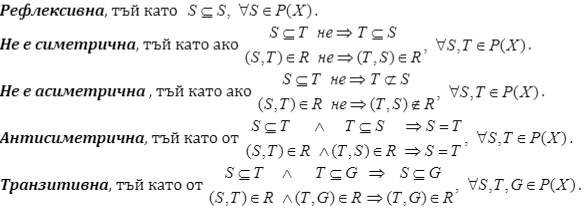
\includegraphics[width=\linewidth]{Pics/Discrete math/ex6/ex6-task1-3.png}
\end{figure}
\end{enumerate}

\subsubsection*{Задача 2}
Нека R и S са релации oт вида
$$R = \{(1, 2), (1, 3), (2, 3), (2, 4), (3, 4) \} \qquad S = \{(2, 1), (3, 1), (3, 2), (4, 2)\}$$
Да се определи композицията им $S \circ R$ \\
Решение \\
$$(b,c) \circ (a,b) = (a,c) $$
$$S \circ R = \{ (1, 1), (1,2), (2, 1), (2, 2) \}$$

\newpage
\subsubsection*{Задача 3}
\begin{figure} [htp!]
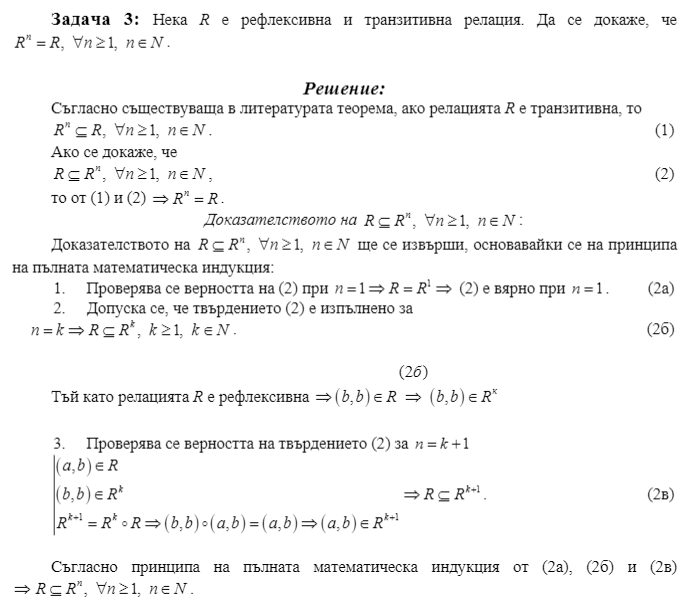
\includegraphics[width=\linewidth]{Pics/Discrete math/ex6/ex6-task3.png}
\end{figure}

\newpage
\subsubsection*{Задача 4}
Да се състави матрица, описваща следната релация R върху множеството \{1,2,3,4\}, където $(a,b) \in R $, тогава и само тогава когато $\vert a - b \vert \leq 1$ \\
Решение : \\
\begin{figure} [htp!]
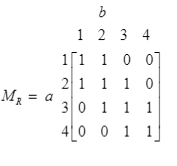
\includegraphics{Pics/Discrete math/ex6/ex6-task4.png}
\end{figure}

\subsubsection*{Задача 5}
Ако релациите R и S се представят със следните матрици
$$M_R = 
\begin{bmatrix}
1 & 0 & 0\\
1 & 1 & 0 \\
1 & 1 & 0 
\end{bmatrix} 
\quad
M_S = 
\begin{bmatrix}
0 & 0 & 1\\
0 & 1 & 0 \\
1 & 1 & 0 
\end{bmatrix}  
$$
Определете матриците, които представят $R \cup S$ и $R \cap S$? \\
Решение: \\
$$
M_{R \cup S} = M_R \lor M_S = 
\begin{bmatrix}
1 & 0 & 1\\
1 & 1 & 0\\
1 & 1 & 0
\end{bmatrix}
\qquad
M_{R \cap S} = M_R \land M_S =
\begin{bmatrix}
0 & 0 & 0\\
0 & 1 & 0\\
1 & 1 & 0
\end{bmatrix}
$$
\newpage
\subsubsection*{Задача 6}
Да се определи релацията по следната матрица
\begin{figure} [htp!]
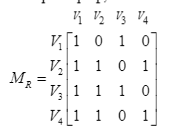
\includegraphics{Pics/Discrete math/ex6/ex6-task6.png}
\end{figure}
$$R = \{(1, 1), (1, 3), (2, 1), (2, 2), (2, 4), (3, 1), (3, 2), (3, 3), (4, 1), (4, 2), (4, 4) \}$$
\subsubsection*{Задача 7}
\begin{figure} [htp!]
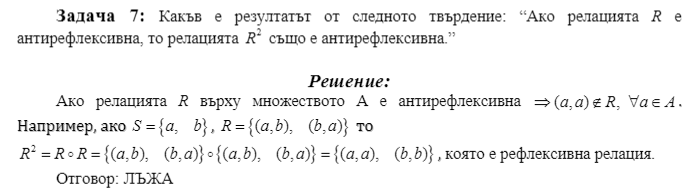
\includegraphics[width=\linewidth]{Pics/Discrete math/ex6/ex6-task7.png}
\end{figure}

\newpage
\section{Упражнение 7: Функции и суми}

\subsubsection*{Задача 1}
Нека са дадени следните множества \\
$
A = \{1, 2, 3, 4\} \\
B = \{ a, b, c\} \\
C = \{2, 7, 10 \}
$\\
На тяхна основа са дефинирани функциите \\
$$g: A \to B \qquad f: B \to C$$
по следния начин
$$g = \{ (1, b), (2, a), (3, c) \} \qquad f = \{ (a, 10), (b, 7), (c, 2) \}$$
Композицията $f \circ g$ е \\
$$ f \circ g = \{ (1, b), (2, a), (3, c) \} \circ  \{ (a, 10), (b, 7), (c, 2) \} = \{ (1, 7), (2, 10), (3, 2) \}$$

\subsubsection*{Задача 2}
Да се намерят обратните функции $f^{-1}$ на следните функции f:
\begin{enumerate}
\item $f: A \to B, \, A = \{ a, b, c \}, \, B = \{2, 7, 10 \}, \, f = \{ (a, 10), (b, 7), (c, 2) \}$
$\forall x \in A \implies \exists y \in B, f(x) = y$\\
f е инекция, f e сюрекция $\implies$ f е биекция $\implies$
$$f^{-1} = \{ (10, a), (7, b), (2, c) \}$$
\item $f: A \to B$, A = \{ Иван, Стоян, Георги, Тони \}, \\
B = \{ Опел, Форд, Рено, Пежо, Ситроен \},\\ 
f= \{ (Иван, Пежо), (Стоян, Форд), (Георги, Рено), (Тони, Опел) \} \\
$\forall a \in A \implies \exists b \in B, f(a) = b$ \\
$f(\varnothing) = \text{Ситроен}$\\
f е инекция, f не e сюрекция $\implies $ f не е биекция$\implies \centernot\exists f^{-1}$ 
\item $f: \mathbb{R} \to \mathbb{R}, \, f(x) = 3x + 5$ \\
f е инекция, f e сюрекция $\implies$ f е биекция $\implies \exists f^{-1}$
$$x = 3y + 5 \implies y = f^{-1}(x) = \frac{x-5}{3} $$
\item $f: \mathbb{R} \to \mathbb{R}, \, x > \frac{2}{7}, \, f(x) = \ln{(7x-2)}$\\
f е инекция, f e сюрекция $\implies$ f е биекция $\implies \exists f^{-1}$
$$x = \ln{(7y-2)} \implies 7y - 2 = e^x \implies y = f^{-1}(x) = \frac{e^x + 2}{7}$$
\end{enumerate}

\subsubsection*{Задача 3}
Да се запишат нулевия, първия, втория и третия член на редица с общ член $a_n$ от вида:
\begin{enumerate}
\item $(-2)^n$\\
$$a_0 = (-2)^0 = 1, \  a_1 = (-2)^1 = -2, \  a_2 = (-2)^2 = 4, \ a_3 = (-2)^3 = -8$$
\item 3\\
$$a_0 = a_1 = a_2 = a_3 = 3$$
\item $7 + 4^n$\\
$$a_0 = 7 + 4^0 = 8, \ a_1 = 7 + 4^1 = 11, \ a_2 = 7 + 4^2 = 23,  \ a_3 = 7 + 4^3 = 71 $$
\item $2^n + (-2)^n$\\
$$a_0 = 2^0 + (-2)^0 = 2 \qquad a_1 = 2^1 + (-2)^1 = 0$$
$$ a_2 = 2^2 + (-2)^2 = 8 \qquad  a_3 = 2^3 + (-2)^3 = 0$$
\end{enumerate}

\subsubsection*{Задача 4}
Да се запише общият член $a_n$ за всеки от посочените редове от цели числа $(n \geq 1, n \in \mathbb{N})$
\begin{enumerate}
\item $ 7, 11, 15, 19, 23, 27, 31, 35, 39, 43, ... $ - аритметична прогресия
$$a_1 = 7 \qquad d = 4 \implies a_n = a_1 +(n-1)d = 7 + (n-1)4$$
\item $ 2, 6, 18, 54, 162, 486, 1458, 4374, 13122, 39366, ... $ - геометрична прогресия
$$a_1 = 2 \qquad q = 3 \implies a_n = a_1 \cdot q^{n-1} = 2 \cdot 3^{n-1}$$
\item $ 3, 6, 11, 18, 27, 38, 51, 66, 83, 102, ... $
$$a_1 = 3 \quad a_2 = 6 = a_1 + 3 \quad a_3 = 11 = a_2 + 5 \quad a_4 = 18 = a_3 + 7$$
$$a_{n-1} = a_{n-2} + (2(n-1) - 1) = a_{n-2} + (2n - 3)$$
$$a_n = a_{n-1} + (2n-1)$$
$$a_n = 3+(3+5+...+(2n-1)) = 2 + (1+3+5+...+(2n-1)) = $$
$$2 + \frac{(1+2n-1)n}{2} = 2 + \frac{2n \cdot n}{2} = n^2 + 2$$
\end{enumerate}

\subsubsection*{Задача 5}
Да се намери стойността на всяка от следните суми:
\begin{enumerate}
\item $S_9 = \sum_{k=0}^8 (1 + (-1)^k)$
$$S_9 = \sum_{k=0}^8 (1 + (-1)^k) = 2 + 0 + 2 + 0 + 2 + 0 + 2 + 0 + 2 = 5 \cdot 2 + 4 \cdot 0 = 10$$
\item $S_4 = \sum_{k=0}^4 (2^k + 3k)$
$$S_4 = \sum_{k=0}^4 (2^k + 3k) = \sum_{k=0}^4 2^k + \sum_{k=0}^4 3k = \sum_{k=0}^4 2^k + 3\sum_{k=0}^4 k$$
$$a_{1geo} \cdot \frac{q^4 - 1}{q -1} + 3 \frac{4(a_{1alg} + a_{4alg})}{2} = 2 \cdot \frac{2^4 - 1}{2 -1} + 3 \frac{4(1 +4)}{2} =  \frac{2 \cdot 15}{1} + \frac{3 \cdot 4 \cdot 5}{2} = 30 + 30 = 60$$
\item $S_5 = \sum_{k=0}^4 5 \cdot 2^k$
$$S_5 = \sum_{k=0}^4 5 \cdot 2^k = 5 \sum_{k=0}^4 2^k = 5 \cdot a_0  \frac{q^5 - 1}{q -1} = 5 \cdot 2^0 \frac{2^5 - 1}{2 -1} = 5 \cdot 31 = 155$$
\item $S = \sum_{i=0}^2 \sum_{j=0}^3 (2i + 3j)$
$$S = \sum_{i=0}^2 \sum_{j=0}^3 (2i + 3j) = \sum_{i=0}^2 \sum_{j=0}^3 2i + \sum_{i=0}^2 \sum_{j=0}^3 3j = $$ $$4 \cdot 2 \sum_{i=0}^2 i + 3 \cdot 3 \sum_{j=0}^3 j = 8 \cdot \frac{(0+2)3}{2} + 9 \cdot \frac{(0+3)4}{2} = 24 + 54 = 78$$
\end{enumerate}

\newpage
\subsubsection*{Задача 6}
\begin{figure} [htp!]
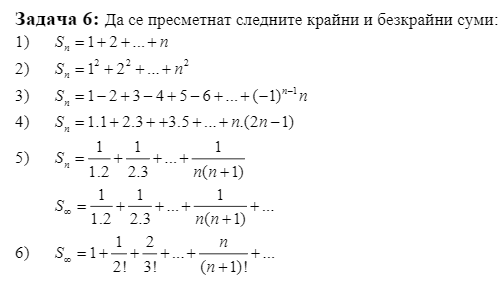
\includegraphics[width = \linewidth]{Pics/Discrete math/ex7/ex7-task6-1.png}
\end{figure}
\begin{figure} [htp!]
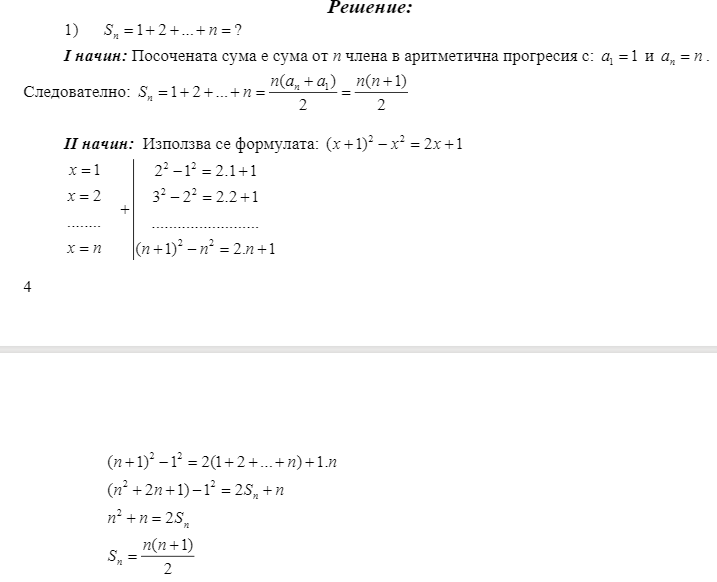
\includegraphics{Pics/Discrete math/ex7/ex7-task6-2.png}
\end{figure}
\begin{figure} [htp!]
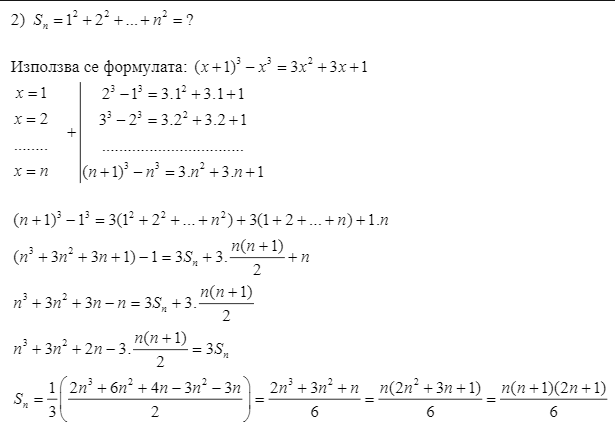
\includegraphics{Pics/Discrete math/ex7/ex7-task6-3.png}
\end{figure}
\begin{figure} [htp!]
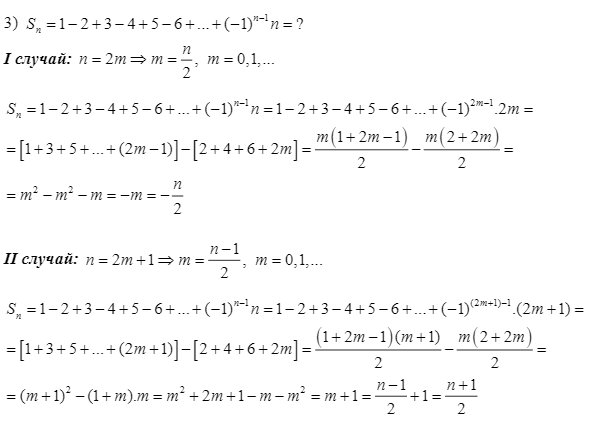
\includegraphics{Pics/Discrete math/ex7/ex7-task6-4.png}
\end{figure}
\begin{figure} [htp!]
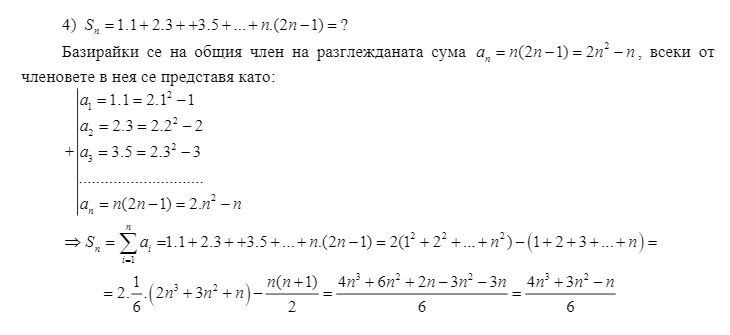
\includegraphics{Pics/Discrete math/ex7/ex7-task6-5.png}
\end{figure}
\begin{figure} [htp!]
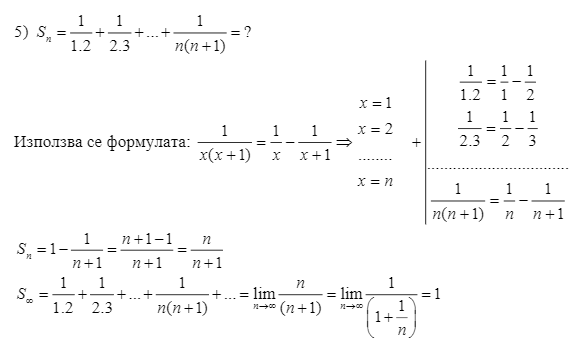
\includegraphics{Pics/Discrete math/ex7/ex7-task6-6.png}
\end{figure}
\begin{figure} [htp!]
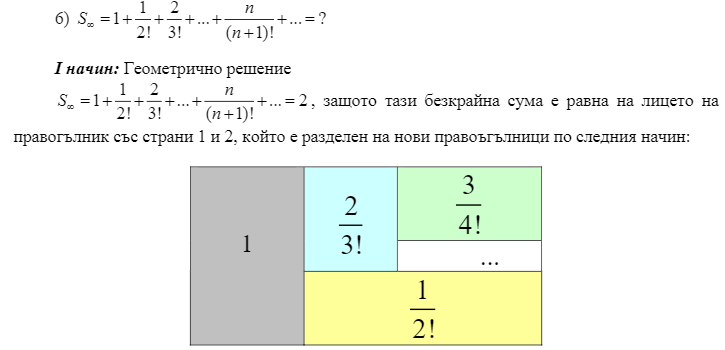
\includegraphics{Pics/Discrete math/ex7/ex7-task6-7.png}
\end{figure}
\begin{figure} [htp!]
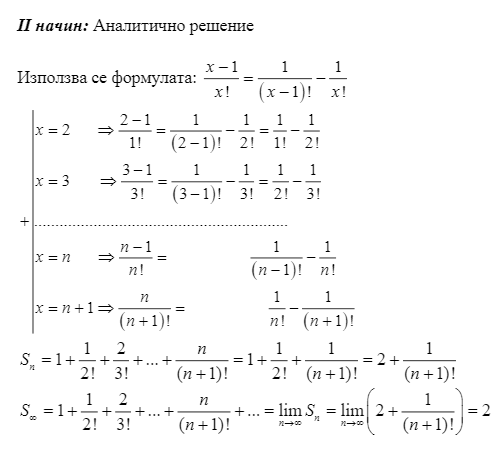
\includegraphics{Pics/Discrete math/ex7/ex7-task6-8.png}
\end{figure}

\newpage
\subsubsection*{Задача 7}
Нека $A = \{3,3,7,15,27 \}$ Да се определи общия член във функцията на индексната променлива $n = \{1,2,3,4,5 \}$.\\
Решение: 
\begin{gather*}
a(n) = an^2 + bn + c \\
\begin{array}{|l@{}}
a(1) = 3 = a \cdot 1^2 + b \cdot 1 + c \\
a(2) = 3 = a \cdot 2^2 + b \cdot 2 + c \\
a(3) = 7 = a \cdot 3^2 + b \cdot 3 + c 
\end{array} \Leftrightarrow 
\begin{array}{|l@{}}
a + b + c = 3\\
4a + 2b + c  = 3\\
9a + 3b + c  = 7
\end{array}\Leftrightarrow  \\
\begin{array}{|l@{}}
c = 3 - a -b\\
4a + 2b + 3 - a -b  = 3\\
9a + 3b + 3 - a -b  = 7
\end{array}\Leftrightarrow  
\begin{array}{|l@{}}
c = 3 - a -b\\
3a + b = 0\\
8a + 2b= 4
\end{array}\Leftrightarrow 
\begin{array}{|l@{}}
c = 3 - a -b\\
b = -3a\\
8a + 2(-3a)= 4
\end{array} \Leftrightarrow  \\
\begin{array}{|l@{}}
8a -6a= 4\\
c = 3 - a -b\\
b = -3a
\end{array} \Leftrightarrow
\begin{array}{|l@{}}
2a= 4\\
c = 3 - a -b\\
b = -3a
\end{array} 
 \Leftrightarrow
\begin{array}{|l@{}}
a= 2\\
b = -3 \cdot 2 = -6\\
c = 3 - 2 -(-6) = 1+6 = 7
\end{array}\\
a(n) = 2n^2 - 6n + 7 
\end{gather*}

\subsubsection*{Задача 8}
Да се намери решението на функцията срямо $y$. 
$$P(x,y) = 7x^2 - 2y^2 = 3$$
Решение: 
\begin{gather*}
7x^2 - 2y^2 = 3\\
2y^2 = 7x^2 - 3 \Leftrightarrow y^2 = \frac{7x^2 - 3}{2} \Leftrightarrow y = \pm \sqrt{\frac{7x^2 - 3}{2}} \\
\frac{7x^2 - 3}{2} \geq 0 \Leftrightarrow 7x^2 - 3 \geq 0 \Leftrightarrow x^2 \geq \frac{3}{7} \Leftrightarrow x \geq \sqrt{\frac{3}{7}} \lor x \leq - \sqrt{\frac{3}{7}}
\end{gather*}
\newpage
\section{Упражнение 8: Графи и дървета}

\subsubsection*{Задача 1}
\begin{figure} [htp!]
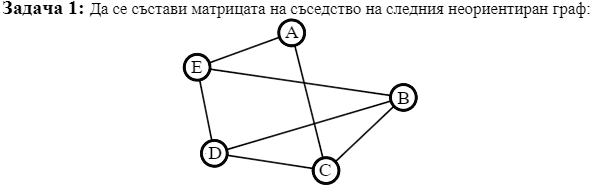
\includegraphics[width = \linewidth]{Pics/Discrete math/ex8/ex8-task1.png}
\end{figure}
$$A_G = 
\begin{bmatrix}
0 & 0 & 1 & 1 & 0 \\
0 & 0 & 1 & 1 & 1 \\
1 & 1 & 0 & 1 & 0 \\
0 & 1 & 1 & 0 & 1 \\
1 & 1 & 0 & 1 & 0 \\
\end{bmatrix}
$$
Извод: Матрицата на съседство на неориентиран граф е симетрична квадратна матрица, чиито елементи $(i,i)$по главния диагонал са 1, ако около съответния връх $V_i$ има примка.
\subsubsection*{Задача 2}
\begin{figure} [htp!]
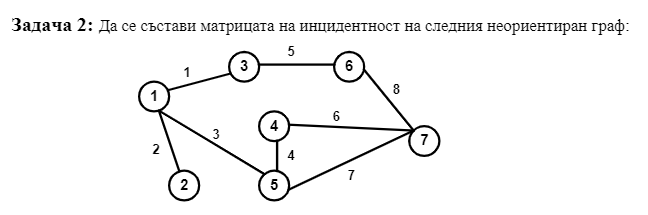
\includegraphics[width = \linewidth]{Pics/Discrete math/ex8/ex8-task2.png}
\end{figure}
$$A_I = 
\begin{bmatrix}
1 & 1 & 1 & 0 & 0 & 0 & 0 & 0 \\
0 & 1 & 0 & 0 & 0 & 0 & 0 & 0 \\
1 & 0 & 0 & 0 & 1 & 0 & 0 & 0 \\
0 & 0 & 0 & 1 & 0 & 1 & 0 & 0 \\
0 & 0 & 1 & 1 & 0 & 0 & 1 & 0 \\
0 & 0 & 0 & 0 & 1 & 0 & 0 & 1 \\
0 & 0 & 0 & 0 & 0 & 1 & 1 & 1 \\
\end{bmatrix}
$$
Извод: Матрицата на инцидентност на неориентиран граф съдържа по две 1 в колона, съответстваща на нормално ребро и по една 1 в колона, съответстваща на ребро-примка.
\subsubsection*{Задача 3}
\begin{figure} [htp!]
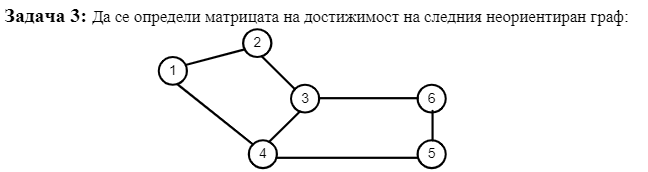
\includegraphics[width = \linewidth]{Pics/Discrete math/ex8/ex8-task3.png}
\end{figure}

\begin{gather*}
I = 
\begin{bmatrix}
1 & 0 & 0 & 0 & 0 & 0 \\
0 & 1 & 0 & 0 & 0 & 0 \\
0 & 0 & 1 & 0 & 0 & 0 \\
0 & 0 & 0 & 1 & 0 & 0 \\
0 & 0 & 0 & 0 & 1 & 0 \\
0 & 0 & 0 & 0 & 0 & 1  \\
\end{bmatrix} 
\quad 
A_G = 
\begin{bmatrix}
0 & 1 & 0 & 1 & 0 & 0 \\
1 & 0 & 1 & 0 & 0 & 0 \\
0 & 1 & 0 & 1 & 0 & 1 \\
1 & 0 & 1 & 0 & 1 & 0 \\
0 & 0 & 0 & 1 & 0 & 1 \\
0 & 0 & 1 & 0 & 1 & 0  \\
\end{bmatrix} 
\quad
H_1 = I \cup A_G = 
\begin{bmatrix}
1 & 1 & 0 & 1 & 0 & 0 \\
1 & 1 & 1 & 0 & 0 & 0 \\
0 & 1 & 1 & 1 & 0 & 1 \\
1 & 0 & 1 & 1 & 1 & 0 \\
0 & 0 & 0 & 1 & 1 & 1 \\
0 & 0 & 1 & 0 & 1 & 1  \\
\end{bmatrix} \\
A_G^2 = A_G \cdot A_G = 
\begin{bmatrix}
0 & 1 & 0 & 1 & 0 & 0 \\
1 & 0 & 1 & 0 & 0 & 0 \\
0 & 1 & 0 & 1 & 0 & 1 \\
1 & 0 & 1 & 0 & 1 & 0 \\
0 & 0 & 0 & 1 & 0 & 1 \\
0 & 0 & 1 & 0 & 1 & 0  \\
\end{bmatrix}
\cdot
\begin{bmatrix}
0 & 1 & 0 & 1 & 0 & 0 \\
1 & 0 & 1 & 0 & 0 & 0 \\
0 & 1 & 0 & 1 & 0 & 1 \\
1 & 0 & 1 & 0 & 1 & 0 \\
0 & 0 & 0 & 1 & 0 & 1 \\
0 & 0 & 1 & 0 & 1 & 0  \\
\end{bmatrix}
= 
\begin{bmatrix}
1 & 0 & 1 & 0 & 1 & 0 \\
0 & 1 & 0 & 1 & 0 & 1 \\
1 & 0 & 1 & 0 & 1 & 0 \\
0 & 1 & 0 & 1 & 0 & 1 \\
1 & 0 & 1 & 0 & 1 & 0 \\
0 & 1 & 0 & 1 & 0 & 1  \\
\end{bmatrix} 
\end{gather*}
\begin{gather*}
A_G^3 = A_G^2 \cdot A_G = 
\begin{bmatrix}
1 & 0 & 1 & 0 & 1 & 0 \\
0 & 1 & 0 & 1 & 0 & 1 \\
1 & 0 & 1 & 0 & 1 & 0 \\
0 & 1 & 0 & 1 & 0 & 1 \\
1 & 0 & 1 & 0 & 1 & 0 \\
0 & 1 & 0 & 1 & 0 & 1  \\
\end{bmatrix} 
\cdot 
\begin{bmatrix}
0 & 1 & 0 & 1 & 0 & 0 \\
1 & 0 & 1 & 0 & 0 & 0 \\
0 & 1 & 0 & 1 & 0 & 1 \\
1 & 0 & 1 & 0 & 1 & 0 \\
0 & 0 & 0 & 1 & 0 & 1 \\
0 & 0 & 1 & 0 & 1 & 0  \\
\end{bmatrix}
= 
\begin{bmatrix}
0 & 1 & 0 & 1 & 0 & 1 \\
1 & 0 & 1 & 0 & 1 & 0 \\
0 & 1 & 0 & 1 & 0 & 1 \\
1 & 0 & 1 & 0 & 1 & 0 \\
0 & 1 & 0 & 1 & 0 & 1 \\
1 & 0 & 1 & 0 & 1 & 0  \\
\end{bmatrix}\\
H_2 = I \cup A_G \cup A_G^2 = H_1 \cup A_G^2 = 
\begin{bmatrix}
1 & 1 & 1 & 1 & 1 & 0 \\
1 & 1 & 1 & 1 & 0 & 1 \\
1 & 1 & 1 & 1 & 1 & 1 \\
1 & 1 & 1 & 1 & 1 & 1 \\
1 & 0 & 1 & 1 & 1 & 1 \\
0 & 1 & 1 & 1 & 1 & 1  \\
\end{bmatrix}\\
H_3 = I \cup A_G \cup A_G^2 \cup A_G^3 = H_2 \cup A_G^3 = 
\begin{bmatrix}
1 & 1 & 1 & 1 & 1 & 1 \\
1 & 1 & 1 & 1 & 1 & 1 \\
1 & 1 & 1 & 1 & 1 & 1 \\
1 & 1 & 1 & 1 & 1 & 1 \\
1 & 1 & 1 & 1 & 1 & 1 \\
1 & 1 & 1 & 1 & 1 & 1  \\
\end{bmatrix}
\end{gather*}
Елементите  на  матрицата $H_3$ са  само  от  1$\implies H_4 = H_3 \implies$ Процедурата  се  спира. \\
Всеки връх от разглеждания граф е достижим от всички останали.

\newpage
\subsubsection*{Задача 4}
\begin{figure} [htp!]
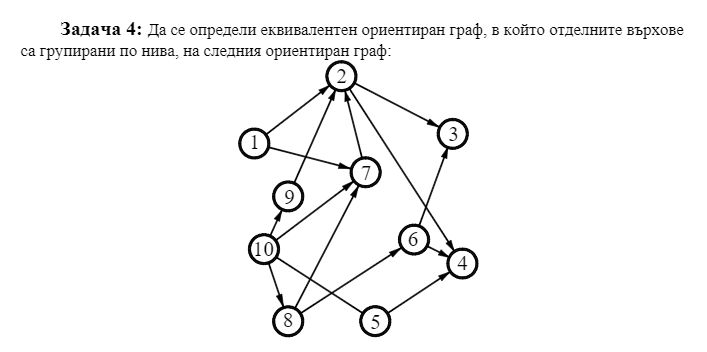
\includegraphics[width = \linewidth]{Pics/Discrete math/ex8/ex8-task4.png}
\end{figure}

\begin{enumerate}
\item За всеки връх $V_i$ се определя	множество $V^+ (i)$ от върхове, всеки от които е начало на дъга, влизаща във върха $V_i$ както следва:
\begin{itemize}
\item $V^+ (1)  = \varnothing $
\item $V^+ (2) = \{ V_1, V_9, V_7 \}$
\item $V^+ (3) = \{ V_2, V_6 \}$
\item $V^+ (4) = \{ V_2, V_5, V_6 \}$
\item $V^+ (5) = \{ V_{10} \}$
\item $V^+ (6) = \{ V_8 \}$
\item $V^+ (7) = \{ V_1, V_10, V_8 \}$
\item $V^+ (8) = \{ V_{10} \}$
\item $V^+ (9) = \{ V_{10} \}$
\item $V^+ (10) = \varnothing $
\end{itemize}
\item Определя се множеството от върхове от нулево ниво, което включва всички висящи (начални) върхове: 
$$V^0 = \{ V_1, V_10\}$$
\item Определя се множеството от върхове от първо ниво, което включва върхове, които са директно свързани чрез дъги единствено с върхове от нулево ниво:
$$V^1 = \{V_9, V_8, V_5 \} \quad V_i \in  V^1 \quad V^+(i) = V_0$$
\item Oпределя се множеството от върхове от второ ниво, което включва върхове, които са директно свързани чрез дъги единствено с върхове от нулево и първо ниво:
$$V^2 = \{V_7, V_6 \} \quad V_i \in  V^2 \quad V^+(i) = V_1$$
\item Определя се множеството от върхове от трето ниво, което включва върхове,които са директно свързани чрез дъги с върхове от нулево, първо и второ ниво:
$$V^3 = \{V_2 \} \quad V_i \in  V^3 \quad V^+(i) = V_2$$
\item Определя се множеството от върхове от четвърто ниво, което включва върхове, които са директно свързани чрез дъги с върхове от нулево, първо, второ и трето ниво:
$$V^4 = \{V_3, V_9 \} \quad V_i \in  V^4 \quad V^+(i) = V_3$$
\item Преномерират се върховете в новия граф (не е задължително).
\end{enumerate}

\begin{figure} [htp!]
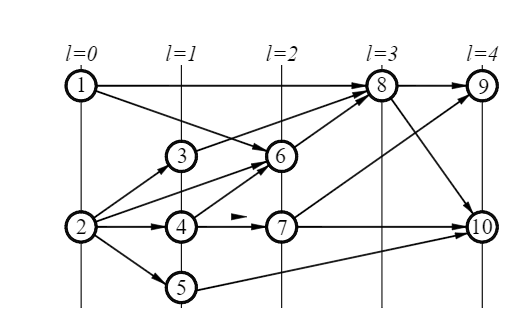
\includegraphics[width = \linewidth]{Pics/Discrete math/ex8/ex8-task4-1.png}
\end{figure}

\newpage
\subsubsection*{Задача 5}
\begin{figure} [htp!]
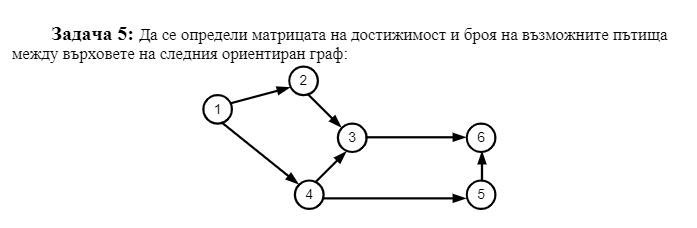
\includegraphics[width = \linewidth]{Pics/Discrete math/ex8/ex8-task5.png}
\end{figure}
\begin{enumerate}
\item Определя се еквивалентния ориентиран граф, в който отделните  върхове са групирани по нива, както следва:
\begin{figure} [htp!]
\centering
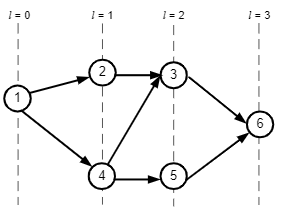
\includegraphics{Pics/Discrete math/ex8/ex8-task5-1.png}
\end{figure}
\item Формира се единична квадратна матрица от вида:
$$
I = 
\begin{bmatrix}
1 & 0 & 0 & 0 & 0 & 0 \\
0 & 1 & 0 & 0 & 0 & 0 \\
0 & 0 & 1 & 0 & 0 & 0 \\
0 & 0 & 0 & 1 & 0 & 0 \\
0 & 0 & 0 & 0 & 1 & 0 \\
0 & 0 & 0 & 0 & 0 & 1  \\
\end{bmatrix} 
\implies \quad 
H^0 = I = 
\begin{bmatrix}
1 & 0 & 0 & 0 & 0 & 0 \\
0 & 1 & 0 & 0 & 0 & 0 \\
0 & 0 & 1 & 0 & 0 & 0 \\
0 & 0 & 0 & 1 & 0 & 0 \\
0 & 0 & 0 & 0 & 1 & 0 \\
0 & 0 & 0 & 0 & 0 & 1  \\
\end{bmatrix} 
$$
\item Формира се матрицата на достижимост до върховете от ниво 1 -$H^1$: 
$$
H^{(0-1)} = 
\begin{bmatrix}
0 & 1 & 0 & 1 & 0 & 0 \\
0 & 0 & 0 & 0 & 0 & 0 \\
0 & 0 & 0 & 0 & 0 & 0 \\
0 & 0 & 0 & 0 & 0 & 0 \\
0 & 0 & 0 & 0 & 0 & 0 \\
0 & 0 & 0 & 0 & 0 & 0  \\
\end{bmatrix}
\implies \quad 
H^1 = H^{(0-1)} = 
\begin{bmatrix}
0 & 1 & 0 & 1 & 0 & 0 \\
0 & 0 & 0 & 0 & 0 & 0 \\
0 & 0 & 0 & 0 & 0 & 0 \\
0 & 0 & 0 & 0 & 0 & 0 \\
0 & 0 & 0 & 0 & 0 & 0 \\
0 & 0 & 0 & 0 & 0 & 0  \\
\end{bmatrix}
$$
\item Формира се матрицата на достижимост до върховете от ниво 2 -$H^2$:
$$
H^{(1-2)} = 
\begin{bmatrix}
0 & 0 & 0 & 0 & 0 & 0 \\
0 & 0 & 1 & 0 & 0 & 0 \\
0 & 0 & 0 & 0 & 0 & 0 \\
0 & 0 & 1 & 0 & 1 & 0 \\
0 & 0 & 0 & 0 & 0 & 0 \\
0 & 0 & 0 & 0 & 0 & 0  \\
\end{bmatrix}
\implies \quad 
H^2 = H^{(1-2)} + H^1 \cdot H^{(1-2)} = 
\begin{bmatrix}
0 & 0 & 2 & 0 & 1 & 0 \\
0 & 0 & 1 & 0 & 0 & 0 \\
0 & 0 & 0 & 0 & 0 & 0 \\
0 & 0 & 1 & 0 & 1 & 0 \\
0 & 0 & 0 & 0 & 0 & 0 \\
0 & 0 & 0 & 0 & 0 & 0  \\
\end{bmatrix}
$$
\item Формира се матрицата на достижимост до върховете от ниво 3 -$H^3$:
$$
H^{(2-3)} = 
\begin{bmatrix}
0 & 0 & 0 & 0 & 0 & 0 \\
0 & 0 & 0 & 0 & 0 & 0 \\
0 & 0 & 0 & 0 & 0 & 1 \\
0 & 0 & 0 & 0 & 0 & 0 \\
0 & 0 & 0 & 0 & 0 & 1 \\
0 & 0 & 0 & 0 & 0 & 0  \\
\end{bmatrix}
\implies \quad 
H^3 = H^{(2-3)} + H^2 \cdot H^{(2-3)} = 
\begin{bmatrix}
0 & 0 & 0 & 0 & 0 & 3 \\
0 & 0 & 0 & 0 & 0 & 1 \\
0 & 0 & 0 & 0 & 0 & 1 \\
0 & 0 & 0 & 0 & 0 & 2 \\
0 & 0 & 0 & 0 & 0 & 1 \\
0 & 0 & 0 & 0 & 0 & 0  \\
\end{bmatrix}
$$
\item Определя се окончателната матрица на достижимост:
$$
H = H^0 \cup H^1 \cup H^2 \cup H^3 = 
\begin{bmatrix}
1 & 1 & 1 & 1 & 1 & 1 \\
0 & 1 & 1 & 0 & 0 & 1 \\
0 & 0 & 1 & 0 & 0 & 1 \\
0 & 0 & 1 & 1 & 1 & 1 \\
0 & 0 & 0 & 0 & 1 & 1 \\
0 & 0 & 0 & 0 & 0 & 1  \\
\end{bmatrix}
$$
\item Определя се броя на възможните пътища между върховете на ориентиранияграф:
$$
H = H^0 + H^1 + H^2 + H^3 = 
\begin{bmatrix}
1 & 1 & 2 & 1 & 1 & 3 \\
0 & 1 & 1 & 0 & 0 & 1 \\
0 & 0 & 1 & 0 & 0 & 1 \\
0 & 0 & 1 & 1 & 1 & 2 \\
0 & 0 & 0 & 0 & 1 & 1 \\
0 & 0 & 0 & 0 & 0 & 1  \\
\end{bmatrix}
$$
\end{enumerate}

\newpage
\subsubsection*{Задача 6}
\begin{figure} [htp!]
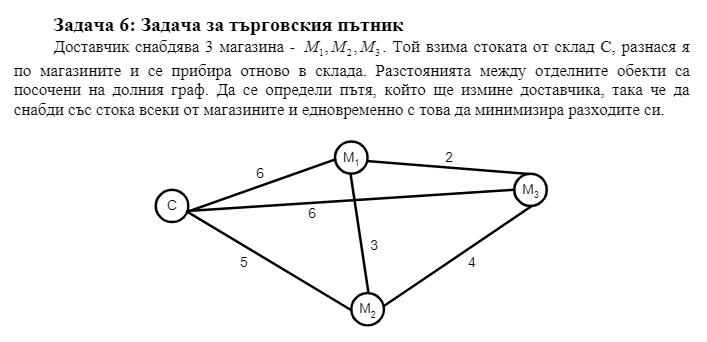
\includegraphics[width = \linewidth]{Pics/Discrete math/ex8/ex8-task6.png}
\end{figure}
Решение: \\
Необходимо е доставчикът да опише т.нар Хамилтонов контур, т.е. тръгвайки от склада С да мине последователно през всеки от магазините само по веднъж и отново да се върне в склада. В случая броя нa върховете на неориентирания граф е $n=4$. Следователно максималният брой различни Хамилтонови контури е $\frac{(n-1)!}{2} = \frac{3!}{2} = 3$, защото:
\begin{enumerate}
\item Фиксира се даден връх за $N_1$.
\item От връх $N_1$ може да се отиде до $(n-1)$ - нови върха, всеки от които може да се означи с връх $N_2$
\item При фиксирани връхове $N_1$ и $N_2$ от връх $N_2$ може да се отиде до $(n-2)$ - нови върха, всеки от които може да се означи с връх $N_1$ и т.н.
\end{enumerate}
$\implies$ Общият брой Хамилтонови контури е $(n-1)!$ -, но всеки два от тях са еднакви, но с противоположна посока на обхождане $\implies$ бщият брой Хамилтонови контури е $\frac{(n-1)!}{2}$.\\
Решението на конкретната задача ще се визуализира чрез моделиране на възможните Хамилтонови контури, използвайки граф-дърво.\\
\begin{figure} [htp!]
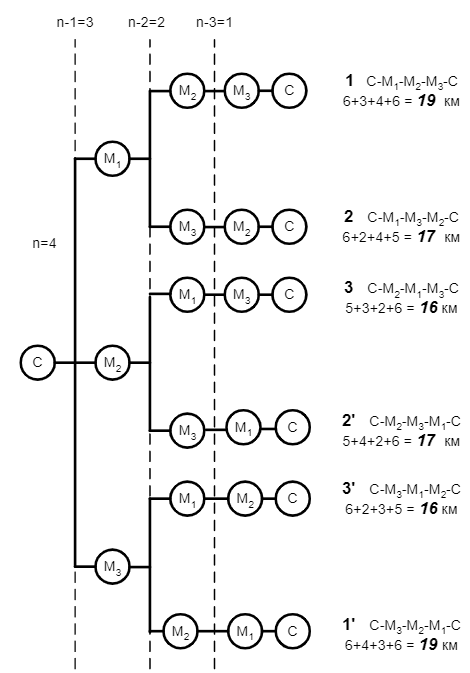
\includegraphics{Pics/Discrete math/ex8/ex8-task6-1.png}
\end{figure}
От дървото се вижда, че двойките контурите 1-1’,  2-2’ и 3-3’ са с равна дължина, но с обратна последователност на обхождане и най-краткият път е 3 (респ.3’),чиято дължина е 16км.

\subsubsection*{Задача 7}
\begin{figure} [htp!]
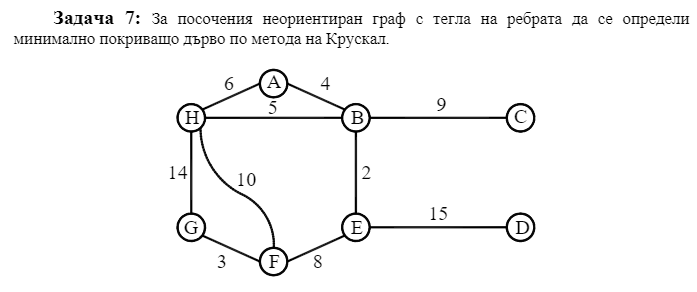
\includegraphics{Pics/Discrete math/ex8/ex8-task7.png}
\end{figure}
Последователността на присвояване на ребра на графа към МПД, съгласно алгоритъма на Крускал е следната: (B, E), (G, F), (A, B), (H,B), (F,E), (B,C), (E,D). \\
Резултантното МПД е показано на следващата фигура:
\begin{figure} [htp!]
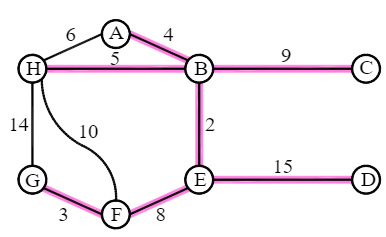
\includegraphics{Pics/Discrete math/ex8/ex8-task7-1.png}
\end{figure}
Съответстващата сума от тегловни коефициентина принадлежащите му ребра, е:
$$ 2 + 3 + 4 + 5 + 8 + 9 + 15 = 46$$
\newpage
\subsubsection*{Задача 8}
\begin{figure} [htp!]
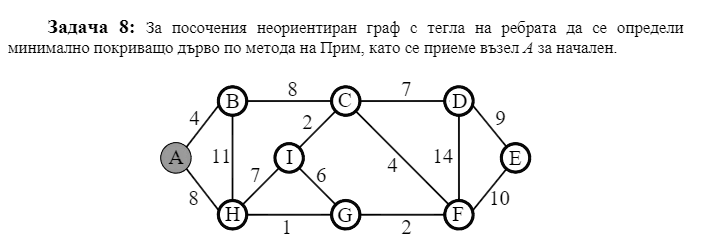
\includegraphics{Pics/Discrete math/ex8/ex8-task8.png}
\end{figure}
\begin{figure} [htp!]
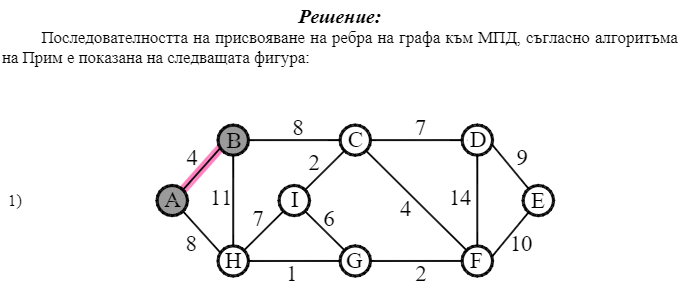
\includegraphics{Pics/Discrete math/ex8/ex8-task8-1.png}
\end{figure}
\begin{figure} [htp!]
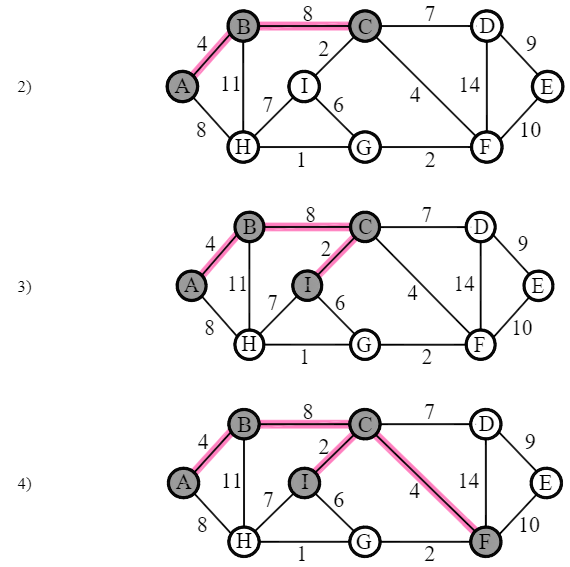
\includegraphics{Pics/Discrete math/ex8/ex8-task8-2.png}
\end{figure}
\begin{figure} [htp!]
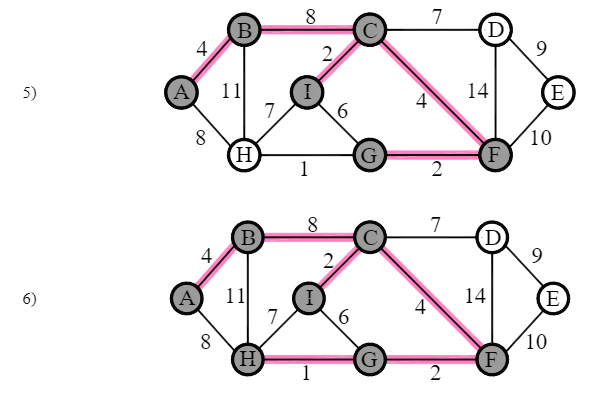
\includegraphics{Pics/Discrete math/ex8/ex8-task8-3.png}
\end{figure}
\begin{figure} [htp!]
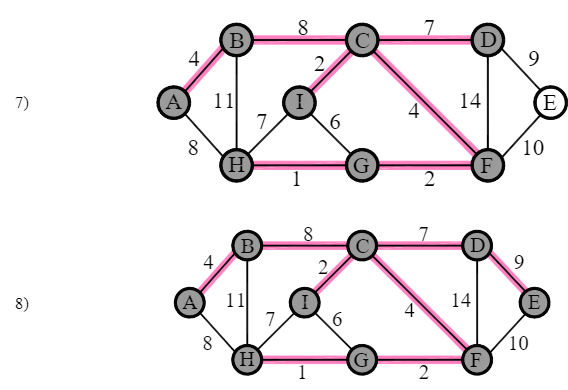
\includegraphics{Pics/Discrete math/ex8/ex8-task8-4.png}
\end{figure}
Съответстващата сума от тегловни коефициентина принадлежащите му ребра, е:
$$ 4 + 8 + 2 + 4 + 2 + 1 + 7 + 9 = 37$$
\newpage
\section{Упражнение 9}

\newpage
\section{ Упражнение 10}

\newpage
\section{ Упражнение 11}

\newpage
\section{ Упражнение 12}

\newpage
\section{ Упражнение 13}
























\end{document}